\documentclass{article}

\usepackage[utf8]{inputenc}
\usepackage[letterpaper, total={6in, 9in}]{geometry}
\usepackage{amsmath}
\usepackage{natbib}
\usepackage{wrapfig}
\usepackage{graphicx}
\usepackage{amssymb}
\usepackage{tikz}

\title{Geometry 5 - 3D Geometry Intro}
\author{TSS Math Club}
\date{Dec 2022}

\begin{document}
\large

\maketitle

\section{3D Geometry: Think 2D}

\subsection{Example}

In a regular tetrahedron $ABCD$, $M$ is the midpoint of $CD$. Find $\angle AMB$.



\tikzset{every picture/.style={line width=0.75pt}} %set default line width to 0.75pt        

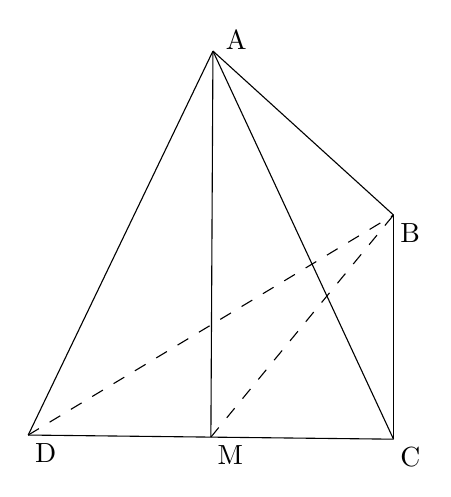
\begin{tikzpicture}[x=0.75pt,y=0.75pt,yscale=-1,xscale=1]
%uncomment if require: \path (0,411); %set diagram left start at 0, and has height of 411

%Straight Lines [id:da34272227772330743] 
\draw    (195.06,89.03) -- (106.06,274.03) ;
%Straight Lines [id:da3339173174782286] 
\draw    (282.06,276.03) -- (106.06,274.03) ;
%Straight Lines [id:da5995848735191855] 
\draw    (195.06,89.03) -- (282.06,276.03) ;
%Straight Lines [id:da28532109602059497] 
\draw    (282.06,168.03) -- (282.06,276.03) ;
%Straight Lines [id:da4649549223878937] 
\draw    (195.06,89.03) -- (282.06,168.03) ;
%Straight Lines [id:da7883950536868969] 
\draw  [dash pattern={on 4.5pt off 4.5pt}]  (106.06,274.03) -- (282.06,168.03) ;
%Straight Lines [id:da8940406459523287] 
\draw  [dash pattern={on 4.5pt off 4.5pt}]  (194.06,275.03) -- (282.06,168.03) ;
%Straight Lines [id:da2799627124005615] 
\draw    (195.06,89.03) -- (194.06,275.03) ;

% Text Node
\draw (200.06,78.03) node [anchor=north west][inner sep=0.75pt]   [align=left] {A};
% Text Node
\draw (284.06,171.03) node [anchor=north west][inner sep=0.75pt]   [align=left] {B};
% Text Node
\draw (284.06,279.03) node [anchor=north west][inner sep=0.75pt]   [align=left] {C};
% Text Node
\draw (108.06,277.03) node [anchor=north west][inner sep=0.75pt]   [align=left] {D};
% Text Node
\draw (196.06,278.03) node [anchor=north west][inner sep=0.75pt]   [align=left] {M};


\end{tikzpicture}\\
Without loss of generality, let the edge-length of $ABCD$ be $2$. It follows that $CM=DM=\sqrt3.$\\
By the Law of Cosines,\[\cos(\angle CMD) = \frac{CM^2 + DM^2 - CD^2}{2(CM)(DM)} = \boxed{\textbf{(B) } \frac13}.\]
\pagebreak

\subsection{Example}
In the diagram, $PABCD$ is a pyramid with square base $ABCD$ and with $PA = PB = PC = PD$.
Suppose that $M$ is the midpoint of $PC$ and that
$\angle BMD = 90^{\circ}$
. Triangular-based pyramid $MBCD$ is
removed by cutting along the triangle defined by the
points $M$, $B$ and $D$. The volume of the remaining
solid $PABMD$ is 288. What is the length of $AB$?



\tikzset{every picture/.style={line width=0.75pt}} %set default line width to 0.75pt        

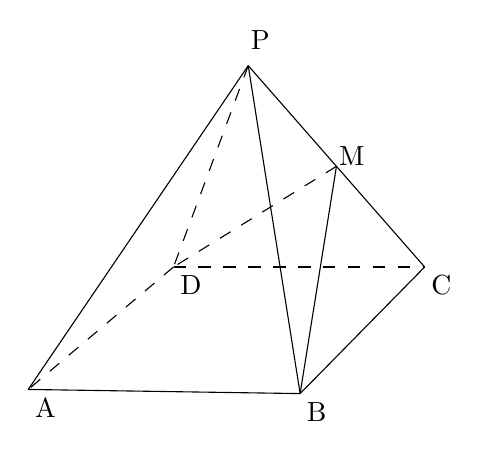
\begin{tikzpicture}[x=0.75pt,y=0.75pt,yscale=-1,xscale=1]
%uncomment if require: \path (0,411); %set diagram left start at 0, and has height of 411

%Straight Lines [id:da06642841678963718] 
\draw    (365.01,240.03) -- (305.01,301.03) ;
%Straight Lines [id:da3133032105153588] 
\draw    (174.01,299.03) -- (305.01,301.03) ;
%Straight Lines [id:da6284514265613841] 
\draw  [dash pattern={on 4.5pt off 4.5pt}]  (244.01,240.03) -- (174.01,299.03) ;
%Straight Lines [id:da23993957607006688] 
\draw    (280.01,143.03) -- (365.01,240.03) ;
%Straight Lines [id:da7607172045026722] 
\draw  [dash pattern={on 4.5pt off 4.5pt}]  (244.01,240.03) -- (365.01,240.03) ;
%Straight Lines [id:da541146629296426] 
\draw    (280.01,143.03) -- (305.01,301.03) ;
%Straight Lines [id:da48648394482635626] 
\draw    (280.01,143.03) -- (174.01,299.03) ;
%Straight Lines [id:da3430468133518938] 
\draw  [dash pattern={on 4.5pt off 4.5pt}]  (280.01,143.03) -- (244.01,240.03) ;
%Straight Lines [id:da3660616410952906] 
\draw  [dash pattern={on 4.5pt off 4.5pt}]  (322.51,191.53) -- (244.01,240.03) ;
%Straight Lines [id:da1892378151273295] 
\draw    (322.51,191.53) -- (305.01,301.03) ;

% Text Node
\draw (176.01,302.03) node [anchor=north west][inner sep=0.75pt]   [align=left] {A};
% Text Node
\draw (307.01,304.03) node [anchor=north west][inner sep=0.75pt]   [align=left] {B};
% Text Node
\draw (367.01,243.03) node [anchor=north west][inner sep=0.75pt]   [align=left] {C};
% Text Node
\draw (246.01,243.03) node [anchor=north west][inner sep=0.75pt]   [align=left] {D};
% Text Node
\draw (280,125) node [anchor=north west][inner sep=0.75pt]   [align=left] {P};
% Text Node
\draw (322.51,180.53) node [anchor=north west][inner sep=0.75pt]   [align=left] {M};


\end{tikzpicture}\\
 Let the side length of the square base $A B C D$ be $2 a$ and the height of the pyramid (that is, the distance of $P$ above the base) be $2 h$.\\
Let $F$ be the point of intersection of the diagonals $A C$ and $B D$ of the base. By symmetry, $P$ is directly above $F$; that is, $P F$ is perpendicular to the plane of square $A B C D$.\\
Note that $A B=B C=C D=D A=2 a$ and $P F=2 h$. \\
We want to determine the value of $2 a$.\\
Let $G$ be the midpoint of $F C$.\\
Join $P$ to $F$ and $M$ to $G$.\\
Consider $\triangle P C F$ and $\triangle M C G$.\\
Since $M$ is the midpoint of $P C$, then $M C=\frac{1}{2} P C$.\\
Since $G$ is the midpoint of $F C$, then $G C=\frac{1}{2} F C$.\\
Since $\triangle P C F$ and $\triangle M C G$ share an angle at $C$ and the two pairs of corresponding sides adjacent to this angle are in the same ratio, then $\triangle P C F$ is similar to $\triangle M C G$.\\
Since $P F$ is perpendicular to $F C$, then $M G$ is perpendicular to $G C$.\\
Also, $M G=\frac{1}{2} P F=h$ since the side lengths of $\triangle M C G$ are half those of $\triangle P C F$.\\
The volume of the square-based pyramid $P A B C D$ equals $\frac{1}{3}\left(A B^2\right)(P F)=\frac{1}{3}(2 a)^2(2 h)=\frac{8}{3} a^2 h$.\\
Triangular-based pyramid $M B C D$ can be viewed as having right-angled $\triangle B C D$ as its base and $M G$ as its height.\\
Thus, its volume equals $\frac{1}{3}\left(\frac{1}{2} \cdot B C \cdot C D\right)(M G)=\frac{1}{6}(2 a)^2 h=\frac{2}{3} a^2 h$.\\
Therefore, the volume of solid $P A B M D$, in terms of $a$ and $h$, equals $\frac{8}{3} a^2 h-\frac{2}{3} a^2 h=2 a^2 h$.\\
Since the volume of PABMD is 288 , then $2 a^2 h=288$ or $a^2 h=144$.\\
We have not yet used the information that $\angle B M D=90^{\circ}$.\\
Since $\angle B M D=90^{\circ}$, then $\triangle B M D$ is right-angled at $M$ and so $B D^2=B M^2+M D^2$.\\
By symmetry, $B M=M D$ and so $B D^2=2 B M^2$.\\
Since $\triangle B C D$ is right-angled at $C$, then $B D^2=B C^2+C D^2=2(2 a)^2=8 a^2$.\\
Since $\triangle B G M$ is right-angled at $G$, then $B M^2=B G^2+M G^2=B G^2+h^2$.\\
Since $\triangle B F G$ is right-angled at $F$ (the diagonals of square $A B C D$ are equal and perpendicular), then
$$
\begin{aligned}
    BG^2 & =B F^2+F G^2=\left(\frac{1}{2} B D\right)^2+\left(\frac{1}{4} A C\right)^2=\frac{1}{4} B D^2+\frac{1}{16} A C^2\\
& =\frac{1}{4} B D^2+\frac{1}{16} B D^2=\frac{5}{16} B D^2=\frac{5}{2} a^2
\end{aligned}
$$
Since $2 B M^2=B D^2$, then $2\left(B G^2+h^2\right)=8 a^2$ which gives $\frac{5}{2} a^2+h^2=4 a^2$ or $h^2=\frac{3}{2} a^2$ or $a^2=\frac{2}{3} h^2$.\\
Since $a^2 h=144$, then $\frac{2}{3} h^2 \cdot h=144$ or $h^3=216$ which gives $h=6$.\\
From $a^2 h=144$, we obtain $6 a^2=144$ or $a^2=24$.\\
Since $a>0$, then $a=2 \sqrt{6}$ and so $A B=2 a=4 \sqrt{6}$.\\
ANSWER: $\boxed{4 \sqrt{6}}$

\pagebreak

\subsection{Example}
Three spheres with radii $11$, $13$, and $19$ are mutually externally tangent. A plane intersects the spheres in three congruent circles centered at $A$, $B$, and $C$, respectively, and the centers of the spheres all lie on the same side of this plane. Suppose that $AB^2 = 560$. Find $AC^2$.\\
\\
Denote by $r$ the radius of three congruent circles formed by the cutting plane. Denote by $O_A$, $O_B$, $O_C$ the centers of three spheres that intersect the plane to get circles centered at $A$, $B$, $C$, respectively.
Because three spheres are mutually tangent, $O_A O_B = 11 + 13 = 24$, $O_A O_C = 11 + 19 = 30$.
We have $O_A A^2 = 11^2 - r^2$, $O_B B^2 = 13^2 - r^2$, $O_C C^2 = 19^2 - r^2$.
Because $O_A A$ and $O_B B$ are perpendicular to the plane, $O_A AB O_B$ is a right trapezoid, with $\angle O_A A B = \angle O_B BA = 90^\circ$.
Hence,\begin{align*} O_B B - O_A A & = \sqrt{O_A O_B^2 - AB^2} \\ & = 4 . \hspace{1cm} (1) \end{align*}
Recall that\begin{align*} O_B B^2 - O_A A^2 & = \left( 13^2 - r^2 \right) - \left( 11^2 - r^2 \right) \\ & = 48 . \hspace{1cm} (2) \end{align*}
Hence, taking $\frac{(2)}{(1)}$, we get\[ O_B B + O_A A = 12 . \hspace{1cm} (3) \]
Solving (1) and (3), we get $O_B B = 8$ and $O_A A = 4$.
Thus, $r^2 = 11^2 - O_A A^2 = 105$.
Thus, $O_C C = \sqrt{19^2 - r^2} = 16$.
Because $O_A A$ and $O_C C$ are perpendicular to the plane, $O_A AC O_C$ is a right trapezoid, with $\angle O_A A C = \angle O_C CA = 90^\circ$.
Therefore,\begin{align*} AC^2 & = O_A O_C^2 - \left( O_C C - O_A A \right)^2 \\ & = \boxed{756}. \end{align*}

\end{document}